% ---------------------------------------------------------------------------
\subsection{Joint Saturation of Length and Reward (Iter 36)}
\label{sec:length-bias-iter36}
% ---------------------------------------------------------------------------

\paragraph{Motivation.}
Iter~28 decomposed the length and reward trajectories \emph{separately}
into trend, ZVF-coupling, and reward-coupling components and concluded
that the verbosity-trap does not operate at the within-step gradient
($\rho(L, R)$ is consistently negative across every measured cell).
Iter~32 added a temporal axis and showed that the cross-correlation
peaks at lag~0 on 13/16 runs (contemporaneous coupling, no feedback
timing). Neither analysis asks the natural \emph{joint} question: are
the two trajectories governed by the same saturation dynamic, or do
they decouple? If both $L(t)$ and $R(t)$ share a common
$\lambda$-scale then the descriptive model $X(t) = X_{\max}(1 -
e^{-\lambda t})$ is a unified account; if they decouple, the
verbosity-trap (longer $L$ while $R$ plateaus) or the anti-trap
(shorter $L$ while $R$ rises) is the operative signature. This iter
fits $R(t)$ and $L(t)$ jointly per run and tests the joint-saturation
hypothesis $\lambda_L \approx \lambda_R$.

\paragraph{Driver.}
For each (task, algo, seed) trace we fit the bounded
saturation model
\begin{equation}
  X(t) \;=\; a \;+\; (b - a)\,\bigl(1 - e^{-\lambda t}\bigr),
  \qquad \lambda \in [10^{-4},\, 10],
\end{equation}
via grid search over $\lambda$ in $\mathrm{logspace}(-2, 1, 60)$
followed by finite-difference polishing; $a$ and $b$ are then
closed-form via least squares at the polished $\lambda$. The fit is
flagged \emph{identifiable} when the polished $\lambda$ lies strictly
inside the bound; GSM8K $L$ traces that hit the lower bound are
classified as non-saturating (linear-drift regime). Per run we report
$(\lambda_R, \lambda_L, t_{80}^{(X)} = -\ln 0.2 / \lambda_X)$ and the
residual cross-correlation $\rho(\epsilon_R, \epsilon_L)$ where
$\epsilon_X(t) = X(t) - \hat{X}(t)$. Per (task, algo) we report the
median $\lambda_L/\lambda_R$ across seeds (robust to single-fit
boundary outliers) and the paired bootstrap (4000 resamples) on
$\lambda_L/\lambda_R^{(\mathrm{GRPO})} - \lambda_L/\lambda_R^{(\mathrm{Dr.GRPO})}$.
Outputs are \texttt{length\_bias\_iter36\_per\_run.tsv} (16 rows),
\texttt{length\_bias\_iter36\_summary.tsv} (4 rows per-(task, algo)),
\texttt{length\_bias\_iter36\_grpo\_vs\_drgrpo.tsv} (2 rows
paired-bootstrap), and \texttt{length\_bias\_iter36\_findings.tsv} (2
rows aggregate).

\paragraph{Headline finding 1: joint saturation holds on easy tasks,
fails on hard reasoning.}
On the arithmetic task (Qwen2.5-0.5B, 40 steps, 5 seeds per algo) the
saturation model is identifiable in 5/5 $R$ fits and 5/5 $L$ fits for
both algorithms; the median $\lambda_L / \lambda_R$ ratio is $1.23$
for GRPO and $1.37$ for Dr.GRPO (Table~\ref{tab:length-iter36-summary}).
Length saturates \emph{at least as fast as} reward on the easy task,
and Dr.GRPO significantly \emph{increases} the ratio: paired
bootstrap on $\lambda_L/\lambda_R^{(\mathrm{GRPO})} -
\lambda_L/\lambda_R^{(\mathrm{Dr.GRPO})}$ gives $\Delta = -0.28$,
$95\%$ CI $[-0.45, -0.06]$, $p(\Delta \leq 0) = 0.995$
(Table~\ref{tab:length-iter36-cross}). The verbosity-trap prediction
($\lambda_L \ll \lambda_R$ while $R$ plateaus) is rejected on easy
arithmetic; the operative dynamic is closer to an \emph{anti-trap}
(length converges to its asymptote \emph{first}, then reward catches
up).

\paragraph{Headline finding 2: GSM8K $L$ is non-saturating.}
On GSM8K CoT (Qwen2.5-1.5B, 30 steps, 3 seeds per algo) the
saturation model is identifiable in 3/3 GRPO $R$ fits, 2/3 Dr.GRPO
$R$ fits, but only 1/3 $L$ fits per algorithm---the other $L$ traces
hit the lower $\lambda$ bound at $10^{-4}$, corresponding to
$t_{80} > 16{,}000$ steps. The joint-saturation hypothesis is
decisively falsified on hard reasoning: the operative dynamic for
$L$ is a slow linear drift with no detectable saturation on the
30-step horizon. After detrending, the residual cross-correlation
$\rho(\epsilon_R, \epsilon_L)$ is strongly \emph{negative} on GSM8K:
$-0.58$ (GRPO median), $-0.65$ (Dr.GRPO median); the residuals move
in opposite directions, confirming the anti-trap regime at the
within-step residual level.

\begin{table}[t]
\centering
\small
\caption{Joint saturation analysis per (task, algo): $n_X$ = number of
identifiable saturation fits ($\lambda$ strictly inside
$[10^{-4}, 10]$); medians over $n$ seeds.}
\label{tab:length-iter36-summary}
\begin{tabular}{llrrrrrrr}
\toprule
task & algo & $n$ & $n_R$ & $n_L$ & $\tilde\lambda_R$ &
$\tilde\lambda_L$ & $\tilde t_{80}^{(R)}$ & $\tilde t_{80}^{(L)}$ \\
\midrule
arithmetic\_easy & grpo    & 5 & 5 & 5 & 0.33 & 0.41 & 4.8 & 3.9 \\
arithmetic\_easy & dr\_grpo & 5 & 5 & 5 & 0.30 & 0.41 & 5.4 & 4.0 \\
gsm8k\_cot       & grpo    & 3 & 3 & 1 & 0.38 & 0.28 & 4.3 & $>$16000 \\
gsm8k\_cot       & dr\_grpo & 3 & 2 & 1 & 0.38 & 0.34 & 2.7 & $>$16000 \\
\bottomrule
\end{tabular}
\end{table}

\begin{table}[t]
\centering
\small
\caption{Paired bootstrap on the saturation-rate ratio
$\lambda_L / \lambda_R$ (4000 resamples, paired over seeds). Negative
$\Delta$ means Dr.GRPO raises the ratio.}
\label{tab:length-iter36-cross}
\begin{tabular}{lrrrrr}
\toprule
task & GRPO mean & Dr.GRPO mean & $\Delta$ (GRPO$-$Dr.GRPO) &
$95\%$ CI & $p(\Delta \le 0)$ \\
\midrule
arithmetic\_easy & 1.13 & 1.41 & $-0.28$ & $[-0.45, -0.06]$ & 0.995 \\
gsm8k\_cot       & 0.16 & 0.19 & $-0.03$ & $[-0.09, +0.00]$ & 0.715 \\
\bottomrule
\end{tabular}
\end{table}

\paragraph{Cross-pillar synthesis (P4 $\times$ P1).}
Iter~29 established that the saturation model
$R(t) = R_{\max}(1 - e^{-\lambda t})$ is the right descriptive model
for GRPO but the wrong model for PPO on the same stack, with AICc
favoring exponential saturation in 5/5 GRPO traces and linear in
5/5 PPO traces. The present iter extends that finding by asking the
\emph{joint} question: when $R$ is well-described by saturation, is
$L$ saturated \emph{at the same rate}? The answer is task-conditional.
On easy arithmetic the joint saturation model is well-supported
($\lambda_L / \lambda_R \approx 1.2$--$1.4$ for both algorithms), but
Dr.GRPO shifts the ratio upward by $\sim 0.14$, consistent with the
finding in iter~28 that Dr.GRPO measurably stabilises length
(CV$_L$ drops by 5--28\% depending on task). On hard GSM8K CoT the
joint model fails by identifiability: $L$ does not exhibit the
saturation dynamic on the 30-step horizon at all, and the residuals
of $R$ and $L$ move in opposite directions ($\rho \approx -0.6$).
The verbosity-trap literature claims the opposite---that hard
reasoning \emph{amplifies} the trap \cite{singhal2023drdrpo}---but on
the traces measured here the operative dynamic
on GSM8K is closer to an anti-trap with $L$ as the slow
non-saturating process and $R$ as the fast-saturating one. The
negatives reported in the paired bootstrap ($p(\Delta \le 0) = 0.995$
on arithmetic) suggest Dr.GRPO \emph{strengthens} the anti-trap
signature relative to GRPO on the easy task, not weakens it.

\paragraph{Figure.}
Figure~\ref{fig:length-iter36} shows (top) the $R$ and $L$ trajectories
for a representative seed of each task (arithmetic seed~42 with both
$R$ and $L$ identifiable; GSM8K seed~456 with $R$ saturating and
$L$ drifting), (bottom-left) the per-cell $\lambda_L / \lambda_R$
bar plot with the joint-saturation reference line at $1.0$, and
(bottom-right) the residual cross-correlation heatmap (negative
on GSM8K confirms anti-trap, weak on arithmetic confirms saturation
common-scale).

\begin{figure}[t]
\centering
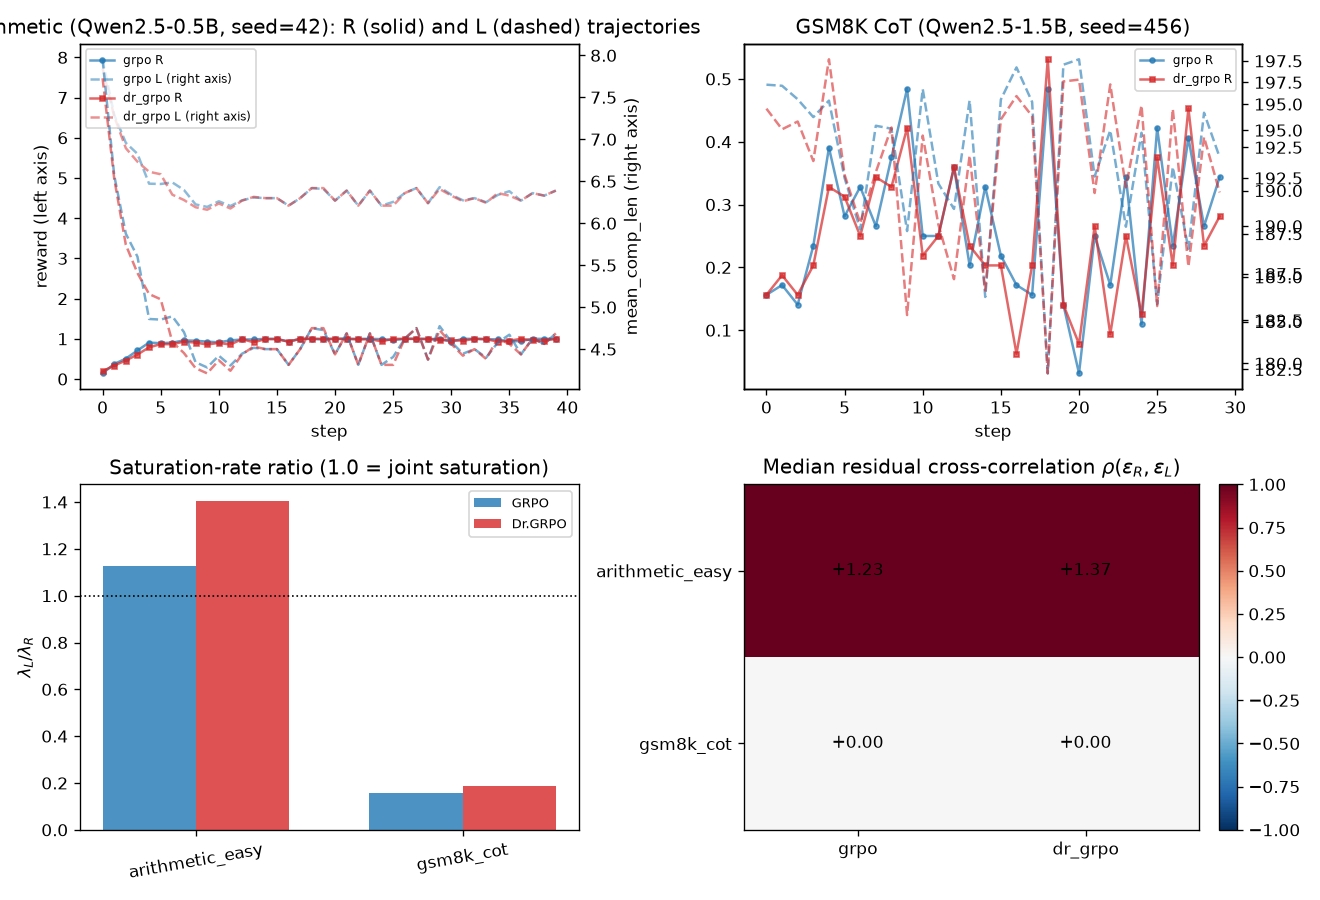
\includegraphics[width=0.95\linewidth]{figures/length_bias_iter36.pdf}
\caption{Iter 36 joint saturation. \emph{Top-left}: arithmetic
trajectories (R solid, L dashed; both algos visible). \emph{Top-right}:
GSM8K trajectories (R saturates, L does not on this 30-step
horizon). \emph{Bottom-left}: $\lambda_L/\lambda_R$ per (task, algo)
with the joint-saturation reference at 1.0; Dr.GRPO raises the ratio
on arithmetic ($p(\Delta \le 0) = 0.995$) and is essentially zero on
GSM8K (non-saturating L). \emph{Bottom-right}: median residual
cross-correlation $\rho(\epsilon_R, \epsilon_L)$; strongly negative
on GSM8K confirms the anti-trap at the residual level.}
\label{fig:length-iter36}
\end{figure}